\documentclass[a4paper,12pt]{memoir}

\newsavebox{\FrontImgBox}
\newlength{\FrontClip}

\usepackage{float}
\usepackage[pdftex]{graphicx}
\usepackage{eso-pic}

% ====== A4 page layout ======
\settypeblocksize{*}{150mm}{1.6}
\setlrmarginsandblock{25mm}{25mm}{*}
\setulmarginsandblock{25mm}{25mm}{*}
\checkandfixthelayout
\usepackage{todonotes}
\pagestyle{empty} % no page number
\usepackage[pdftex]{graphicx}
\usepackage{eso-pic}

 \usepackage{microtype} % better justification & protrusion
\usepackage{newtxtext} % Times-like body text (newspaper vibe)
\usepackage[scaled]{helvet} % Sans for headlines and decks
\usepackage[T1]{fontenc}
\usepackage[utf8]{inputenc}
\usepackage{tikz}
\usetikzlibrary{decorations.text}

% ====== Columns & visuals ======
\usepackage{multicol}
\setlength{\columnsep}{0.28in}
\setlength{\columnseprule}{0.2pt}

\usepackage{graphicx}
\usepackage{wrapfig}
\usepackage{caption}
\captionsetup{font=small,labelfont=bf}

\usepackage[dvipsnames]{xcolor}
\usepackage{lettrine} % drop caps
\usepackage[many]{tcolorbox} % pull quotes / sidebars
%\usepackage[print,1to1]{booklet} %print option switches to landscape
%\pagespersignature{16}
\usepackage{pgfplots}
\pgfplotsset{width=10cm,compat=1.9}

\tcbset{
  colback=black!2,
  colframe=black!40,
  boxsep=4pt, left=6pt, right=6pt, top=6pt, bottom=6pt,
  sharp corners,
}

\usepackage{caption}
\captionsetup[figure]{labelformat=empty}

% ====== Headings & bylines ======
\setsecheadstyle{\Large\bfseries\sffamily}
\setsubsecheadstyle{\normalsize\bfseries\sffamily}
\setsubsubsecheadstyle{\normalsize\itshape}

\newcommand{\kicker}[1]{\textsf{\bfseries\small\color{Gray} #1}}
\newcommand{\headline}[1]{\textsf{\bfseries\fontsize{34}{36}\selectfont #1}}
\newcommand{\deck}[1]{\textsf{\large\itshape #1}}
\newcommand{\byline}[1]{\textsf{\small\color{Gray} Af #1}}
\usepackage{tikz}
\usetikzlibrary{fadings,patterns}

% Define a generic "fade to transparent" around a rectangle
\tikzfading[name=image fade,
  inner color=transparent!50,
  outer color=transparent!100]

  % Text outline ("border around letters")
\usepackage{contour} % works with pdfLaTeX/XeLaTeX/LuaLaTeX
\contourlength{0.9pt}         % default stroke thickness
\contournumber{32}            % smoothness of the outline

% Helpers: white text with dark outline (and a thinner variant)
\newcommand{\ow}[2][black]{\contour{#1}{\textcolor{white}{#2}}}
\newcommand{\owthin}[2][black]{%
  \begingroup\contourlength{0.6pt}\contour{#1}{\textcolor{white}{#2}}\endgroup}

% ====== Page banner / folio ======
\makepagestyle{newspaper}
\makeoddhead{newspaper}{\textsf{\small Den Rullende Sten}}{}{\textsf{\small Sponsoreret af Det Glemte Akademi}}
\makeevenhead{newspaper}{\textsf{\small Sponsoreret af Det Glemte Akademi}}{}{\textsf{\small Den Rullende Sten}}
\makeoddfoot{newspaper}{}{\textsf{\small\thepage}}{}
\makeevenfoot{newspaper}{}{\textsf{\small\thepage}}{}
\makeheadrule{newspaper}{\textwidth}{0.4pt}
\pagestyle{newspaper}

% ====== Pull quote and sidebar environments ======
\newenvironment{pullquote}
  {\begin{tcolorbox}[enhanced, breakable]\itshape\large}
  {\end{tcolorbox}}


\usepackage{xparse}
\usepackage{wrapfig}

% Justérbare standarder for sidebar i spalter
\newcounter{sidebarlines}              % hvor mange linjer der skal "wrappe" forbi boksen
\setcounter{sidebarlines}{14}
\setlength{\sidebarwidth}{0.42\columnwidth}

\newcommand{\godentry}[5]{%
% #1 = placering, #2 = titel, #3 = billedfil, #4 = side l/r, #5 = tekst
\begin{wrapfigure}{#4}{0.24\columnwidth}
  \vspace{-8pt}
  \centering
  \includegraphics[width=0.20\columnwidth]{#3}
  \vspace{-12pt}
\end{wrapfigure}

\subsection*{#1. #2}
#5

\par\medskip
}

% ====== Utilities ======
\newcommand{\separator}{%
  \par\noindent{\color{black!40}\rule{\textwidth}{0.4pt}}\par
}


% Front feature image: spans \textwidth, keeps aspect ratio, fades at edges,
% and overlays outlined text (no boxes).
% Usage: \FrontFeatureImage{<image>}{<kicker>}{<headline>}{<deck>}{<credit>}
\newcommand{\FrontFeatureImage}[5]{%
  % Typeset image at \textwidth just once and measure its height
  \sbox{\FrontImgBox}{\includegraphics[width=\textwidth]{#1}}%
  % Total height of the scaled image (height + depth)
  \dimen0=\dimexpr\ht\FrontImgBox+\dp\FrontImgBox\relax
  % Max allowed height
  \dimen2=.8\textheight
  % Choose visible height: min(actual, max)
  \ifdim\dimen0>\dimen2
    \setlength{\FrontClip}{\dimen2}%
  \else
    \setlength{\FrontClip}{\dimen0}%
  \fi
  %
  \begin{tikzpicture}
    % Define a "frame" we’ll use for anchors & clipping
    \coordinate (TL) at (0,0);                       % top-left
    \coordinate (TR) at (\textwidth,0);              % top-right
    \coordinate (BL) at (0,-\FrontClip);             % bottom-left (cropped)
    \coordinate (BR) at (\textwidth,-\FrontClip);    % bottom-right (cropped)

    % Image with soft fading edges, clipped to the frame (crops from the bottom)
    \begin{scope}
      \clip (TL) rectangle (BR);
      \node[anchor=north west, inner sep=0pt,
            path fading=image fade, fit fading=false] at (TL)
        {\usebox{\FrontImgBox}};
    \end{scope}

    % Dark wash for legibility, also softly faded (match the same clip)
    \begin{scope}
      \clip (TL) rectangle (BR);
      \fill[black,opacity=0.30, path fading=image fade] (BL) rectangle (TR);
    \end{scope}

    % Text stack (bottom-left) — outline style preserved
    \node[anchor=south west, xshift=1em, yshift=1em, align=left,
          text width=.75\textwidth] at (BL){%
      \sffamily
      % Kicker (optional)
      \if\relax\detokenize{#2}\relax\else
        {\owthin[black!85]{\textsf{\bfseries\small #2}}}\\[0.15em]\fi
      % Headline
      {\ow{\bfseries
        \resizebox{1\textwidth}{!}{#3}%
      }}\\[0.2em]
      % Deck
      {\owthin{\large\itshape #4}}%
    };

    % Credit (bottom-right), small outline
    \node[anchor=south east, xshift=-1em, yshift=1em] at (BR)
      {\sffamily\small \owthin[black!85]{#5}};
  \end{tikzpicture}%
}


\newenvironment{infobox}[1]
{\begin{tcolorbox}[
  title=\textsf{\bfseries #1},
  colback=black!3,
  colframe=black!65,
  fonttitle=\small,
  fontupper=\small,
  boxsep=4pt,
  left=5pt,
  right=5pt,
  top=5pt,
  bottom=5pt,
  sharp corners
]}
{\end{tcolorbox}}

\newcommand{\paragraf}[1]{%
  \par\medskip
  \noindent\textbf{\S#1:}%
}
 

\begin{document}
%\pdfpageheight=\paperwidth
%\pdfpagewidth=\paperheight
%\paperwidth=\pdfpagewidth
%\paperheight=\pdfpageheight 
% ====== Nameplate ======
\begin{figure}
  \begin{center}
      
\includegraphics[width=0.98\textwidth]{Logo.png}%
  \end{center}    
\end{figure}
\begin{center}
  {\Large\sffamily Udgave 133}
\end{center}


% Front feature image (keeps aspect ratio, spans \textwidth)
\FrontFeatureImage{Fælles.png}
{ESSELAIA OG MORWEN DØD!}
{FREDENS GUDINDE OG DØDENS GUDINDE ER VÆK!}
{Alle i sorg! (Undtaget sortelevere)}
{}

\vspace{.75\baselineskip}
\newpage  

% ====== Lead story (Front page) ======
\par\medskip 
\headline{TO GUDINDER DRÆBT!} 
\par\medskip 
\deck{Esselaia og Morwen er faldet og Kalish mærker allerede følgerne} 
\par\medskip 
\byline{Redaktionen} 
\medskip 
\lettrine[lines=2,lhang=0.1,loversize=0.05]{E}{sselaia og Morwen} er døde. Fredens, naturens og dragernes gudinde samt dødens, tidens og skatternes gudinde er blevet dræbt af Gudestenene. 

\par\medskip 

Ifølge de første beretninger blev de frygtede Gudesten brugt under angrebet, men hvem der udførte dette angreb vides endnu ikke. Gudestenene er de samme kræfter, som tidligere blev brugt til at dræbe Daikia. Myndighederne har endnu ikke fremlagt en samlet forklaring på, hvordan to gudinder kunne falde på samme dag, men det var velkendt at disse to gudinder stod tæt sammen, og mentes at være den tætteste alliance blandt guderne.

\par\medskip 

Esselaia var engang et menneske og en druide, der kom til A'kastin efter Almans død. Hendes lære handlede om fred, kærlighed og forståelse, selv mellem gamle fjender. Den Vandrende ophøjede hende, så hun kunne hjælpe med at genoprette den balance, som var gået tabt med Alman. Siden blev hun kendt som Dragernes Dronning og Den Barmhjertige. 

\par\medskip 

Morwen var engang sortelver, men blev siden ophøjet til gudinde, hvorefter hun blev dræbt af Ilsherne. Som Ærkedæmon blev hun derefter endnu engang ophøjet til gudinde, denne gang gudinde. Denne gang vogtede hun over døden og tiden, beskyttede de dødes sjæle og opretholdt den orden, som skatter, gæld, kontrakter og handel byggede på. 

\par\medskip 

Sammen dømte Esselaia og Morwen de døde. Esselaia førte Skæbnens tråd, mens Morwen syede med Tidens nål. Hvor den ene så det gode, så den anden det onde. Først sammen kunne de se en hel sjæl. Nu er begge dommersæder tomme, og ingen er sikre på hvordan de undgår Sjælenes Malstrøm.

\par\medskip 

Morwens død har også skabt panik blandt økonomer og handelsfolk. I en verden, hvor alkymister kan fremstille guld af bly og Troldmænd skabe Mitril af Jern, har rigdom aldrig kun været et spørgsmål om sjældne metaller. Det var Morwens guddommelige vilje, der gav vægt til mønter, priser, gæld og løfter. 

\par\medskip 

Den kejserlige mønt forsikrer, at én Fjend fortsat er én Fjend. Alligevel har flere vekselerere lukket deres boder, og købmænd er begyndt at kræve betaling i korn, jern eller andre varer, som ikke kan fremstilles i en alkymists kolbe. Prisen på brød siges allerede at variere fra gade til gade. 

\par\medskip 

Samtidig står dragerne uden deres dronning, druiderne uden deres beskytter og freds kontrakter uden nogen guddommelig opbakning, hvilket ikke virker godt for borgerkrigen i Permersland. Ingen ved endnu, hvad der sker med de sjæle, som venter på deres dom. 

\par\medskip 

Der cirkulerer allerede rygter om urolige drager, ure der går baglæns, mønter der ændrer vægt, og døde der ikke kan finde videre. Redaktionen har endnu ikke kunnet bekræfte disse beretninger. 

\par\medskip 

Kalish har mistet guder før. Men aldrig før har verden på samme dag mistet freden, dommen over de døde og den guddommelige orden bag sin økonomi. 

\par\medskip 

Ét er sikkert: Vi har endnu ikke set den katastrofe som venter.


\section*{Nyheder}

\subsection*{Drageæg forsvundet!} 
Vi har tidligere rapporteret om drageægget i Salezstads zoologiske have. Nu er det forsvundet. Ingen ved, hvor det er blevet af, og mange frygter, at forsvindingen hænger sammen med Esselaias død og dragernes pludselige mangel på en dronning.

\section*{Politik}

\subsection*{\HUGE Blod på Den Røde Trone}
\par\medskip
\deck{Hvordan Aurelia Fjendebane mistede en far, en bror, en nevø og en niece, men vandt et imperium}
\par\medskip
\byline{Stefani Ervind}
\medskip


\lettrine[lines=4,lhang=0.1,loversize=0.05]{D}{er} er sorg ved hoffet, siges det. Naturligvis er der det. Men det er ikke kun sorg ved hoffet, når nogen dør i den rigtige rækkefølge. Kejserinde Aurelia Fjendebane bærer efter sigende sin sorg med værdighed. Det fortæller hoffets skrivere os i hvert fald, og de ville naturligvis aldrig pynte på noget så alvorligt som en kejserlig families private lidelser. Hun sørger over sin fader, Erik Fjendebane den Anden. Hun sørger over sin broder, Conrad Fjendebane. Hun sørger sikkert også over den besynderlige omstændighed, at Conrads børn ikke længere står i vejen for hendes krav på tronen.
\begin{wrapfigure}{r}{0.42\columnwidth}
\begin{infobox}{DEN RØDE TRONE}
Den Røde Trone er Imperiets kejserlige sæde og symbolet på Fjendebane-slægtens magt.
\end{infobox}
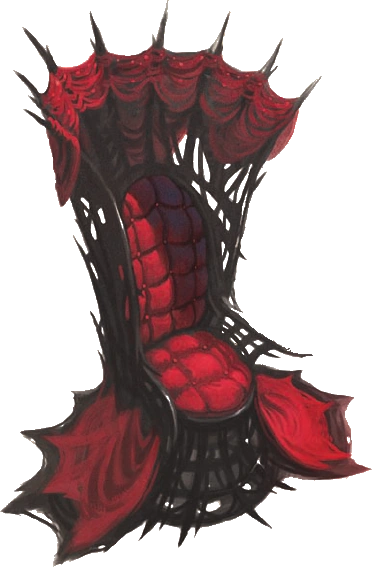
\includegraphics[width=0.4\columnwidth]{Tronen.png}
\caption{Den Røde Trone}
\end{wrapfigure}
Det sidste nævnes sjældent.

Den officielle forklaring er nydelig nok. Erik faldt ved Sydporten efter at have været i kamp med Conrad. Conrad faldt ligeledes i skyggen af samme katastrofe. Conrads børn, ramt af sorg og hellig vrede, valgte derefter at dedikere sig til Kelllwan Kirken og afstod dermed fra Den Røde Trone. Aurelia, som før alt dette stod fjerde i arverækken, blev "modvilligt" nødt til at tage kronen på for rigets skyld.

En smuk fortælling. Og hvis du spørger denne rapporter, er det en for smuk fortælling.

Det mest interessante er måske ikke engang, at Aurelia endte med kronen. Det interessante er, hvor hurtigt alle omkring hende blev enige om, at det ikke var mærkeligt. Der var ingen langvarig offentlig strid om Conrads børns rettigheder. Ingen stor adelssamling, hvor loyalister krævede, at de unge arvinger blev ført frem. Ingen højlydt konflikt mellem Kelllwan Kirken og hoffet, som om de to arvinger var betaling for Kirkens stilhed.

Men hvad førte til Erik og Conrads død? Vi har før populiceret en sang skrevet af en skjald som så hvad der skete ved Sydpoten. Den sang, der nu cirkulerer blandt soldater og krofolk, fremstiller Conrad som en søn, der advarede sin fader, og som blev mødt med hån. Hvis sangen er bare halvt sand, stod Conrad ikke uden ære. 

Derfor er det værd at spørge, hvem der havde fordel af at gøre Conrad vred, ustabil eller besværlig i folkets øjne. En som måske ikke var så sikker på at Conrad ville forsvinde ved Sydporten?

Kelllwan Kirken står også i en besynderlig behagelig position. Den har fået Conrads børn i sin varetægt, eller i hvert fald under sin åndelige vejledning, og samtidig har den fået en kejserinde, hvis tronkrav kun er rent, så længe de samme børn ikke længere gør krav på noget.

Nogle læsere vil sikkert kalde denne artikel respektløs. Andre vil sige, at man ikke bør mistænkeliggøre en sørgende kejserinde uden beviser. Til det svarer jeg, at imperier sjældent har brug for beviser for at lave deres egne anklager.

Måske er Aurelia Fjendebane blot en ulykkelig kvinde, der bar kronen, fordi ingen anden kunne. Måske er Conrads børn helt frivilligt gået ind i Kelllwans tjeneste. Måske var Sydporten en tragedie uden hænder bag tæppet og uden adelige, der skiftede loyalitet som vinden blæser.

Men i så fald må vi lykønske kejserinden.

\par\medskip

\textit{Redaktionen gør opmærksom på, at vrede breve fra hoffet, Kelllwan Kirken eller bekymrede Aurelia-tilhængere modtages med glæde. Svar trykkes i næste udgave mod sædvanligt gebyr på 15 Fjend.}
\separator


\section*{Kultur \& Tro}

\subsection*{\HUGE Den Store Rangliste}
\par\medskip
\deck{Hvem den mest populære gud i Kalish?}
\par\medskip
\byline{Broder Anselm, gæsteskribent}
\medskip

\lettrine[lines=3,lhang=0.1,loversize=0.05]{D}{e} lærde ved Det Glemte Akademi har i årevis diskuteret, hvilke guder der egentlig står stærkest i folkets hjerter. Redaktionen har derfor foretaget en undersøgelse blandt præster, lejesvende, og drukkenbolte.

Resultatet er denne rangliste over rigets mest omtalte guddomme. 

Har du en anden oplevelse? Hvorfor ikke skrive til os med din mening!

\separator
\par\medskip

\textbf{\Large 11. Den Navnløse - Gudernes Gud}
\par

Selv guderne taler sjældent om dem direkte. Og det siges at kende navnet på denne gud skal man betale med sin sindstilstand. 

De står over guderne som den højeste magt, baggrunden til ordenen blandt guderne og den kraft, som selv de mægtigste må bøje sig for. Denne gud har ingen præster og lader til at sove. Ingen kender noget til dem, men guderne ved denne overgud holder dem på plads.

Guden lader endda til at være todelt, med en del der hærsker fra den øverste Sfære, og en der hærsker fra Dæmonernes Sfære.

\par\medskip
\textbf{\Large 10. Carmenor - Den Første Dværg Gud}
\par

Dværgenes gamle gud og engang hersker over deres folk. I dag nævnes han mest i gamle sange og sørgmodige fortællinger. Hans fald gav plads til stærkere kræfter, og selv blandt dværgene er hans navn begyndt at samle støv. Carmenor blev dræbt af Daikia's børn: Ilsherne.

Et sørgeligt eftermæle, men dog et værdigt et.

\begin{figure}[H]
  \begin{center}
  
\includegraphics[width=0.33\columnwidth]{CarmenorLogo.jpg}
  \end{center}
  \caption{Det ældste skjold fundet med Carmenors symbol. Dette har nok inspireret Nordlands symbol.}
\end{figure}

\par\medskip
\textbf{\Large 9. Alman - Den Naturens Gud}
\par
Naturens vogter og elementernes gamle herre. I modsætning til mange andre guder søgte Alman hverken krig eller storhed. Hans død efterlod dog verden langt mere ustabil, end mange ønsker at indrømme. Alman blev dræbt af Ballator, da sønnen af Hadets Ærkedæmon startede Dæmonkrigen.

Han mindes stadig af nogen folk, men det er ikke alle der kender til denne gamle gud, og du finder ingen præster for en gud som ikke kan give dem.

\begin{figure}[H]
  \begin{center}
    
\includegraphics[width=0.33\textwidth]{alman.jpg}
  \end{center}
    \caption{Alman's symbol}
\end{figure}

\par\medskip
\textbf{\Large 8. Daikia - Mørkets moder}
\par

Sortelvernes gamle gudinde og ophav til meget af den uro, verden stadig mærker efterdønningerne af. Hendes tilhængere frygtede hende næsten lige så meget, som de tilbad hende. Hun blev dræbt af Raffael Moordet.

Der findes stadig folk, der hvisker hendes navn om natten. Det siges endda at der også er en gruppe af sortelevere som ikke har opgivet at tilbede hende.
\begin{figure}[H]
  \begin{center}
    
\includegraphics[width=0.15\textwidth]{Daikia.png}
  \end{center}
  \caption{Daikia's Symbol}
\end{figure}

\par\medskip
\textbf{\Large 7. Ewen - Visdommens Herre}
\par

Magiens vogter og de lærdes store beskytter. Ewen elsker viden, diskussioner og mysterier, som ingen andre helt forstår endnu.

Præsterne siger, at han søger sandheden i alt.

Kritikere siger, at han kan formå at gøre enhver løsning til et problem.

\begin{figure}[H]
  \begin{center}
    
\includegraphics[width=0.33\textwidth]{Ewen.jpg}
  \end{center}
  \caption{Ewen's Symbol}
\end{figure}
\par\medskip

\textbf{\Large 6. Raffael Moordet - Skyggernes Fyrste}
\par

Tyvenes, løgnernes og dæmonernes mester. En nederdrægtig og lumsk figur, som selv de mægtigste guder har prøvet at tage livet af. Den sidste der prøvede var Daikia, og Raffael Moordet brugte Sjælenes Malstrøm og Gudestenene til at dræbe hende.

Hans præster lover frihed, magt og hemmelig viden. Vi kan kun anbefale at lade være med at tale med dem.

\begin{figure}[H]
  \begin{center}
    
\includegraphics[width=0.33\textwidth]{RaffaelSymbol.png}
  \end{center}
  \caption{Raffael Moordet's Symbol}
\end{figure}
\par\medskip

\textbf{\Large 5. Orlek - Krigens Brøl}
\par

Grønhudernes gud og den levende ånd af kamp, styrke og erobring. Orlek gør intet halvt. Hvis noget er værd at gøre, er det værd at gøre med blod på øksen.

Overraskende mange følger ham frivilligt.

\begin{figure}[H]
  \begin{center}
    
\includegraphics[width=0.33\textwidth]{OrlekSymbol.jpg}
  \end{center}
  \caption{Orlek's Symbol}
\end{figure}
\par\medskip


\textbf{\Large 4. Morwen - Dødens Dronning} 
\par Morwen var gudinde for døden, tiden, skatterne og den orden, der holdt Kalishs økonomi sammen. Hun var blandt de yngste gudinder, men nåede på kort tid at blive en fast del af både begravelser, kontrakter, gældsbreve og kejserlige skattekontorer. 

I en verden, hvor troldmænd og alkymister kan skabe guld, var det Morwens vilje, der sikrede, at værdi var mere end blot skinnende metal. En mønt var en mønt, en gæld var en gæld, og en underskrevet aftale betød noget. 

Hun modsatte sig desuden nekromanti og vanærelse af de døde. Det gjorde hende upopulær blandt nekromantikere og ganske populær blandt næsten alle andre. 

Efter hendes død virker syvendepladsen næsten beskeden. 

\begin{figure}[H] 
  \begin{center} 
    
\includegraphics[width=0.33\textwidth]{MorwenSymbol.png} 
  \end{center} 
  \caption{Morwens Symbol} 
\end{figure}

\par\medskip
\textbf{\Large 3. Esselaia - Fredens Vogter}
\par

Den nyligt dræbte gudinde for drager, kærlighed, fred og elementerne. Hun prædikede fred, forståelse og troen på, at selv gamle fjender kunne finde fælles grund. 

Det gjorde hende enten til den viseste blandt guderne eller den mest optimistiske. Efter hendes død må Kalish nu finde ud af, om hendes lære kan overleve uden hende.

\begin{figure}[H]
  \begin{center}
      
\includegraphics[width=0.33\textwidth]{Esselaia Symbol full.png}
  \end{center}  
  \caption{Esselaia's Symbol}
\end{figure}


\textbf{\Large 2. Ishtar - Den Førstefødte}
\par

Sortelvernes store dronning og en tidligere Halv-overgud som har nedværdiget sig selv til \underline{kun} at være gudinde. Loyalitet, styrke og lydighed er hendes idealer, og hendes folk følger hende med næsten skræmmende hengivenhed.

Selv hendes fjender omtaler hende med respekt, især fordi hende og hendes brødre, ilsherne, er kendt for at dræbe guder som en hobby.

\begin{figure}[H]
  \begin{center}
    
\includegraphics[height=0.15\textheight]{Ishtar.png}
  \end{center}
  \caption{Ishtar's Symbol}
\end{figure}
\par\medskip

\textbf{\Large 1. Kelllwan - Kongen på Tronen}
\par

Gudernes konge, beskytter af familier, smede og lov. Kelllwan er den type gud, der forventer orden, loyalitet og styrke af sine tilhængere.

Han er respekteret af næsten alle. Og hans messias, Refulsit Lux, er kendt for sin autoritære hengivelse til loven.

\begin{pullquote}  
I en landsby nær Nordlands sydgrænse blev messiasen gjort opmærksom på, at et barn havde stjålet brød fra et tempel. Præsterne bad om nåde og forklarede, at barnets familie var døde under dæmonernes hærgen.

Messiasen lod barnet fremføre for sig og spurgte kun ét spørgsmål:

“Vidste du, at det var forbudt?”

Da barnet nikkede, lod messiasen straffen fuldbyrde offentligt, og Messiasen var selv bødlen da barnet skulle henrettes.
\end{pullquote}

\begin{figure}[H]
  \begin{center}
    
\includegraphics[width=0.33\textwidth]{KelllwanSymbol.png}
  \end{center}
  \caption{Kelllwan's Symbol}
\end{figure}

\separator

\par\medskip

\textit{Redaktionen gør opmærksom på, at flere kirker allerede har sendt vrede breve vedrørende denne rangliste. Dette tager vi som et tegn på journalistisk succes.}

\section*{Bekendtgørelser}

\subsection*{Fra Imperiets Lovkontor}

\textit{Følgende bekendtgørelser er fremsendt til redaktionen under kejserligt segl. Redaktionen har valgt at trykke dem i fuld længde, da bøden for ikke at gøre det var nok til at bygge en ny Sydport.}

\par\medskip

\begin{infobox}{NYE LOVE FRA IMPERIET}
Ved kejserlig myndighed, i Kejserinde Aurelia Fjendebanes navn, bekendtgøres følgende nødvendige love for rigets sikkerhed.
\end{infobox}

\subsection*{Kirkelov MXII: Om guddommelige dødsfald}

\paragraf{1} Alle borgere pålægges straks at indrapportere tegn på dæmoniske manifestationer til nærmeste tempel, kaserne eller embedsmand. Dette er for at imødekomme en potentiel ny trussel.

\paragraf{2} Det er forbudt uden tilladelse at erklære en gud for død, udød, genfødt eller ophøjet.

\paragraf{3} Overtrædelse straffes med bøde, offentlig irettesættelse eller henrettelse.

\subsection*{Arbejderloven XXII: Om Sydportens Arbejdspligt}

\paragraf{1} Alle raske borgere inden for tre dagsrejser af Sydporten kan pålægges midlertidig arbejdspligt til genopbygning af rigets sydlige forsvar.

\paragraf{2} Fritagelse kan gives til:
\begin{itemize}
  \item børn under sværdhøjde,
  \item døde borgere med bekræftet attest fra Morwen Kirken (Dette inkludere ikke de udøde borgere),
  \item personer i aktiv kamp mod dæmoner,
  \item adelige.
\end{itemize}

\paragraf{3} Arbejde udført under Kelllwan Kirkens opsyn tæller som både samfundspligt og moralsk forbedring. Løn udbetales efter gældende takster.

\subsection*{Provinslov VI: Om navne og byer}

\paragraf{1} Alle offentlige kort, tavler og handelsdokumenter skal fremover indeholde plads til mulige fremtidige navneændringer af byer, fæstninger og særligt symbolske steder.

\paragraf{2} Spørgsmålet om Marcusstads/Dorianborgs eventuelle omdøbning er endnu ikke afgjort, men borgere mindes om, at højlydt modstand mod navneændringer kan tolkes som mangel på taknemmelighed over for rigets helte.

\subsection*{Handelslov XIV: Om private valutaer og møntens fortsatte værdi} 

\paragraf{1} Handelskompagni Guld, herefter omtalt som HKG, må ikke præsenteres som kejserlig mønt, Fjend eller anden guddommeligt sikret valuta. 

\paragraf{2} Alle kompagnier, laug og private handelsordninger skal tydeligt oplyse, om en betaling kan bruges til at købe brød, betale gæld og indfri skat. 

\paragraf{3} Handelskompagniet kan fortsat betale medarbejdere i HKG, da det anses som arbejderens eget ansvar at efterspørge betaling, som også har værdi uden for Handelskompagniets egne boder. 

\paragraf{4} Den kejserlige mønt Fjend har efter Morwens død fortsat præcis den værdi, som Imperiet erklærer, at den har. 

\paragraf{5} Guld fremstillet gennem alkymi, trolddom, bøn, forbandelser eller anden unaturlig værdiskabelse skal deklareres ved enhver handel og kan ikke anvendes til skattebetaling uden kejserligt stempel. 

\paragraf{6} Det er forbudt at hæve priser alene med begrundelsen: ``Gudinden er død.'' 

\paragraf{7} Det er ligeledes forbudt at opkøbe hele landsbyers beholdning af korn, salt eller jern med henblik på senere videresalg under en formodet økonomisk undergang. 

\paragraf{8} Overtrædelse straffes med bøde i rigtig valuta. Lovkontoret afgør på betalingstidspunktet, hvad der tæller som rigtig valuta.

\newpage
\section*{Muntre Indslag}
\subsection*{Sang: Røvfar}
Tekst: Svarre

\begin{figure}[H]
  \centering
  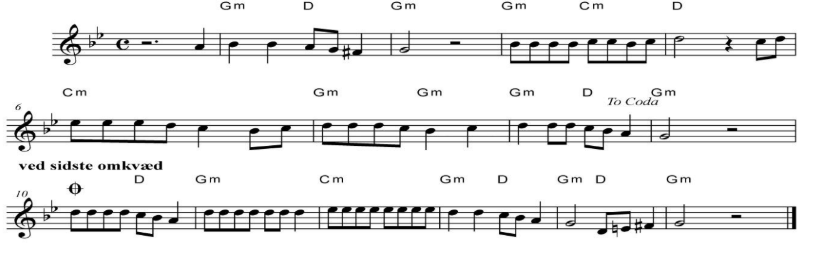
\includegraphics[width=0.98\textwidth]{Røvfar.png}
\end{figure}

\begin{multicols}{2}
\raggedcolumns

\noindent Omkv)\\
Når Røvfar leger sin leg\\
Bli’r din fremtid meget sort for dig\\
Når dit liv det går amok\\
Og du indser, du’ et pjok,\\
Så’ det Røvfar, der leger sin leg

\medskip

\noindent 1)\\
Hvis du vil tænde, ild når du går\\
Men flammen sætter ild til dit hår\\
Og du under host og hark\\
Troede du sku’ ryg’ tobak\\
Ødelægger piben som du fik i går

\medskip

\noindent Omkv)\\
Når Røvfar leger sin leg\\
Så bli’r din rygrad blød som bolledej\\
Når dit liv er gået amok\\
Og du indser, du’ et pjok\\
Er det røvfar, der leger sin leg

\medskip

\noindent 2)\\
Hvis det regner, når du går hjem fra kroen\\
Og du ved, at du skal hjem og slå’s af konen\\
Hele lønnen den gik nøel\\
For du brugte den på øl\\
Og så falder du så i en mudderpøl

\medskip

\noindent Omkv)\\
Så det Røvfar der leger sin leg\\
Håbet bliver sortere end beg\\
Når dit liv er gået amok\\
Og du prygles af en stok\\
Er det Røvfar, der leger sin leg

\medskip

\noindent 3)\\
Hvis du falder over dine egne ben\\
Og knalder hovedet ned i en sten\\
Og du slår dit knæ af led\\
Og du lander på et sted\\
Der hvor koen lige før stod og sked

\medskip

\noindent Omkv)\\
Er det Røvfar der leger sin leg\\
Jeg har aldrig sagt, du ikke er et kvaj\\
Du ka' lisså godt indse det:\\
Du ka' ikk' gør' noet ve' det\\
Er det røvfar der leger sin leg

\medskip

\noindent 4)\\
VI ved jo godt han vinder til sidst\\
Han slukker glædens allersidste gnist\\
Du bør altid vær på vagt\\
Han har nye planer lagt\\
Og så har han nærmest uindskrænket magt

\medskip

\noindent Omkv)\\
For røvfar leger sin leg\\
Din fremtid den bliver meget sort for dig\\
Når liv er gået amok\\
Vil du indse du’ et pjok\\
Fordi Røvfar leger sin\\
Virk’lig vir’klig leger sin\\
Det er her du bli’r til grin\\
Og jeg kalder dig et svin\\
Når Røvfar leger sin leg\\
Dideli-daj

\end{multicols}

\newpage

\begin{figure}[H]
  \centering
  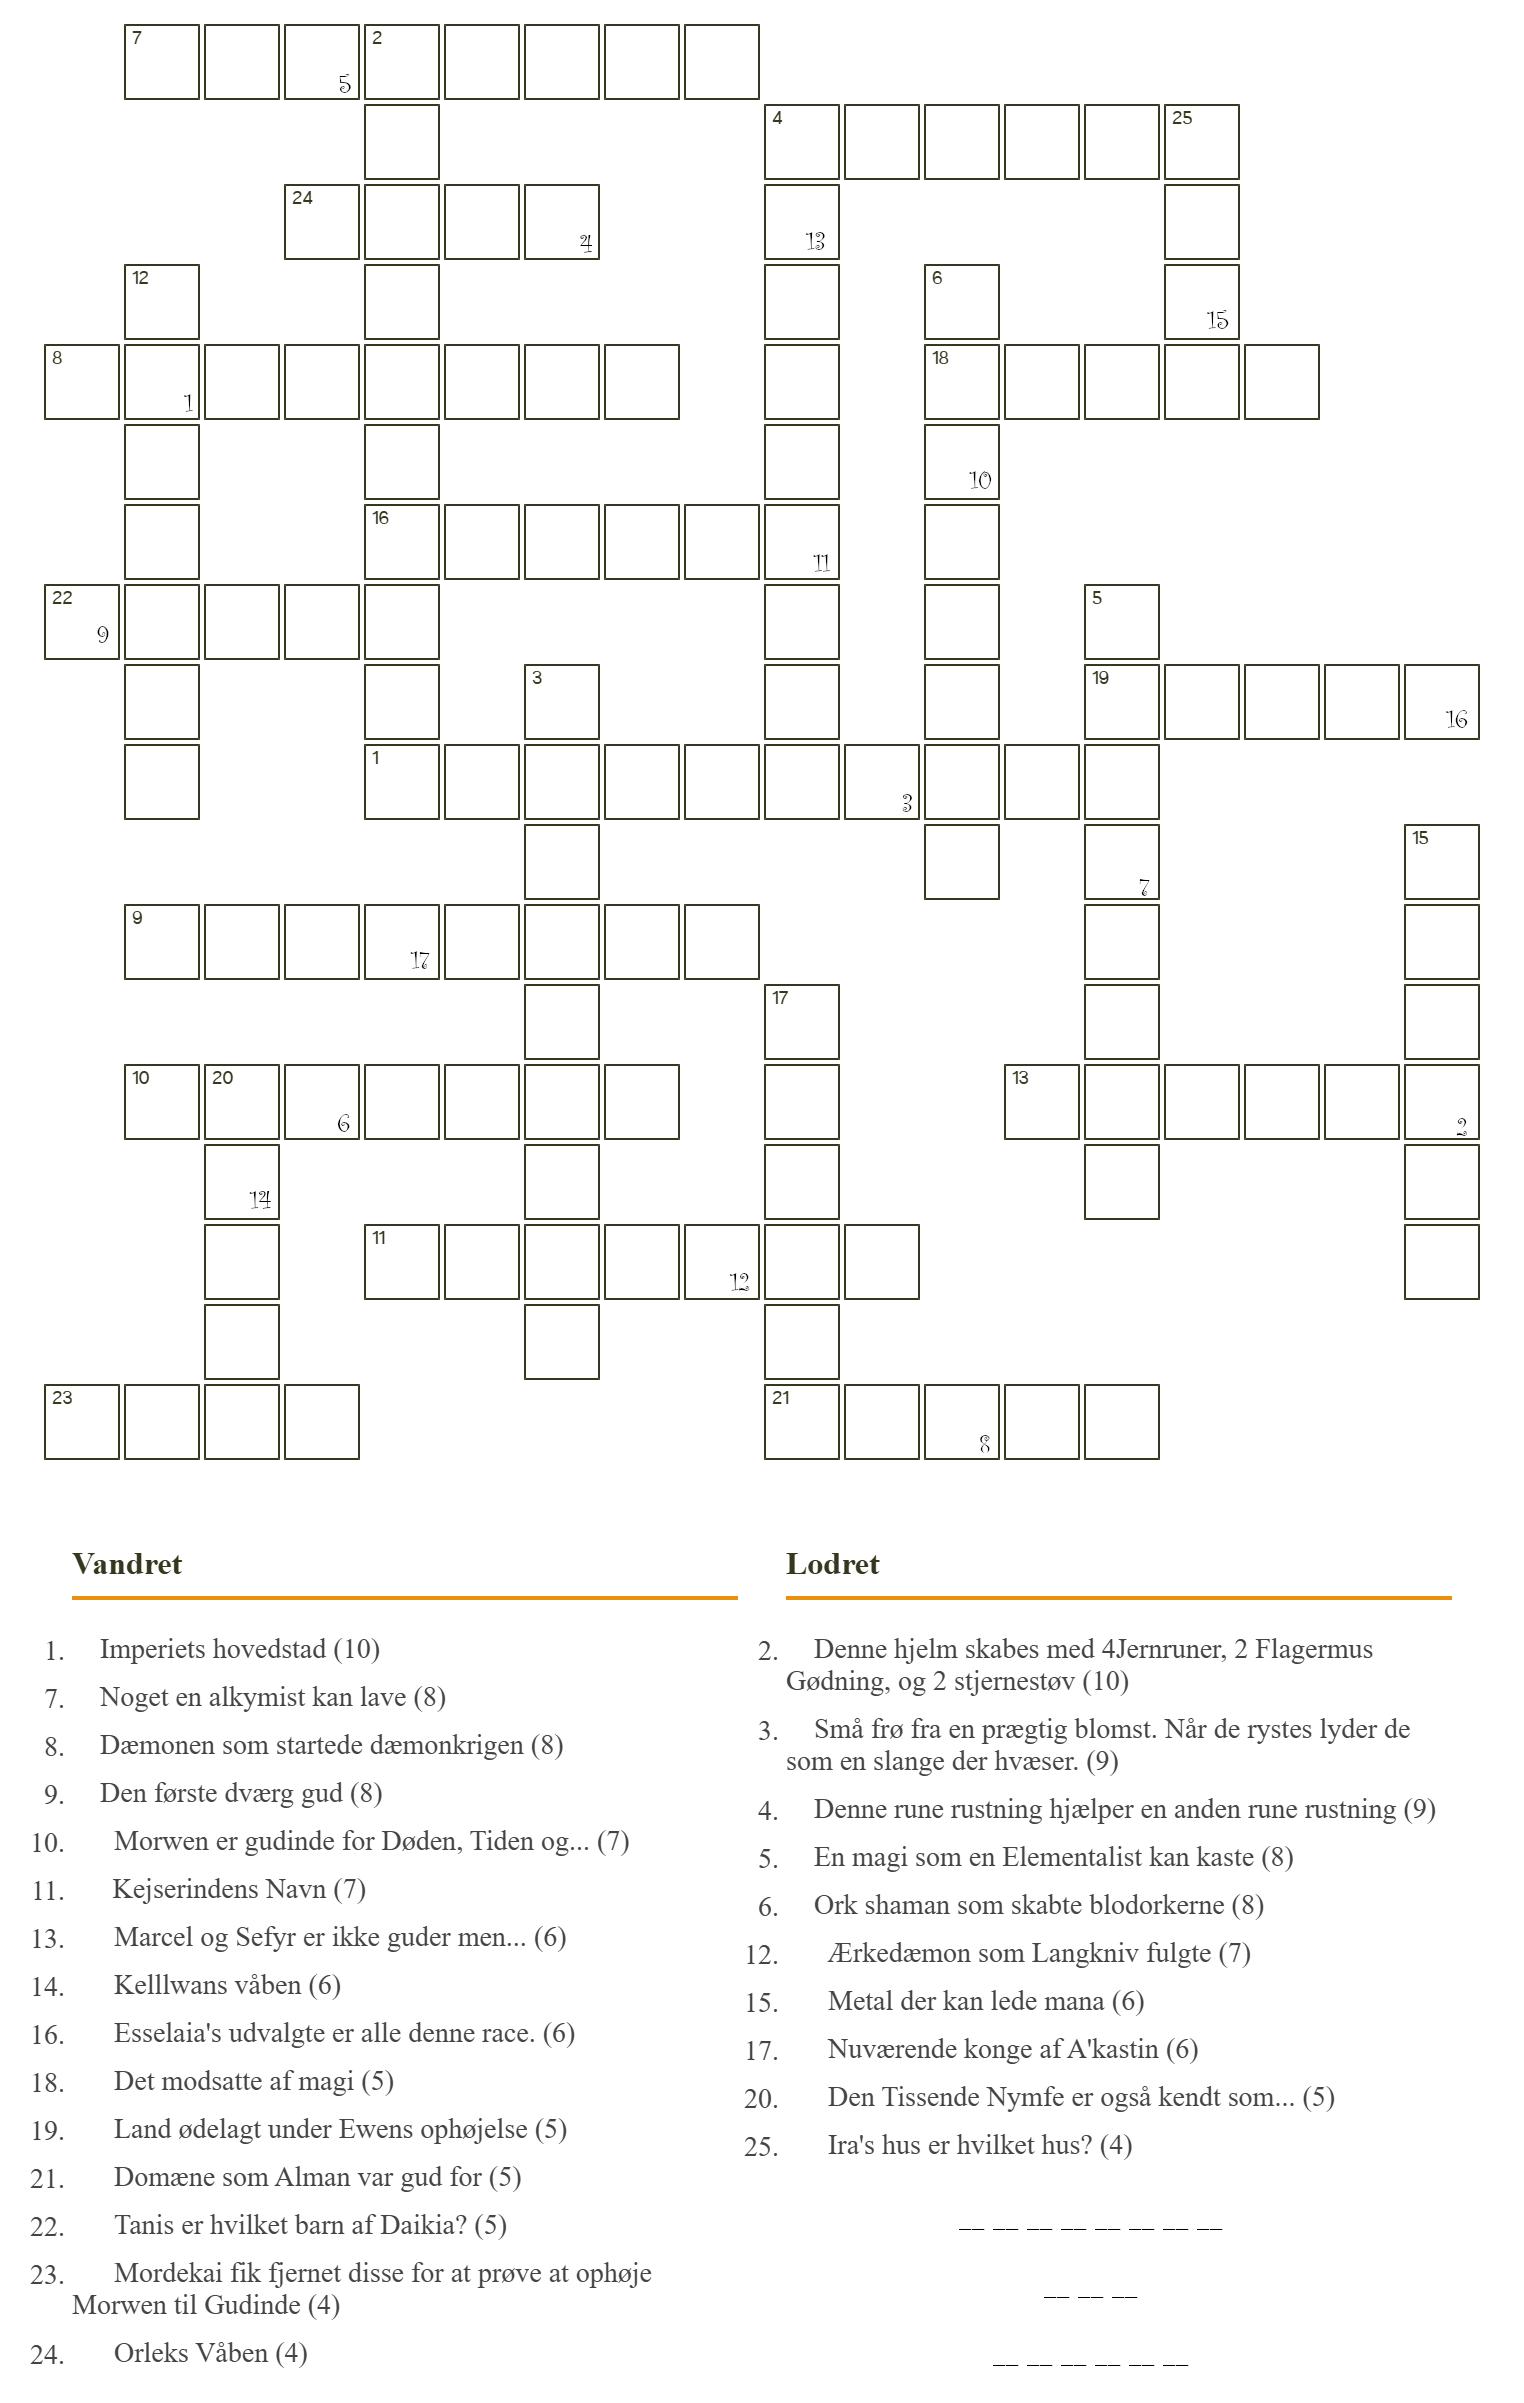
\includegraphics[width=\textwidth]{krydsord1-Blank.png}
\end{figure}
\newpage


\section*{Reklamer}
\subsection*{BRING JERN! OG SULFUR!}
\begin{figure}[H]
  \centering
  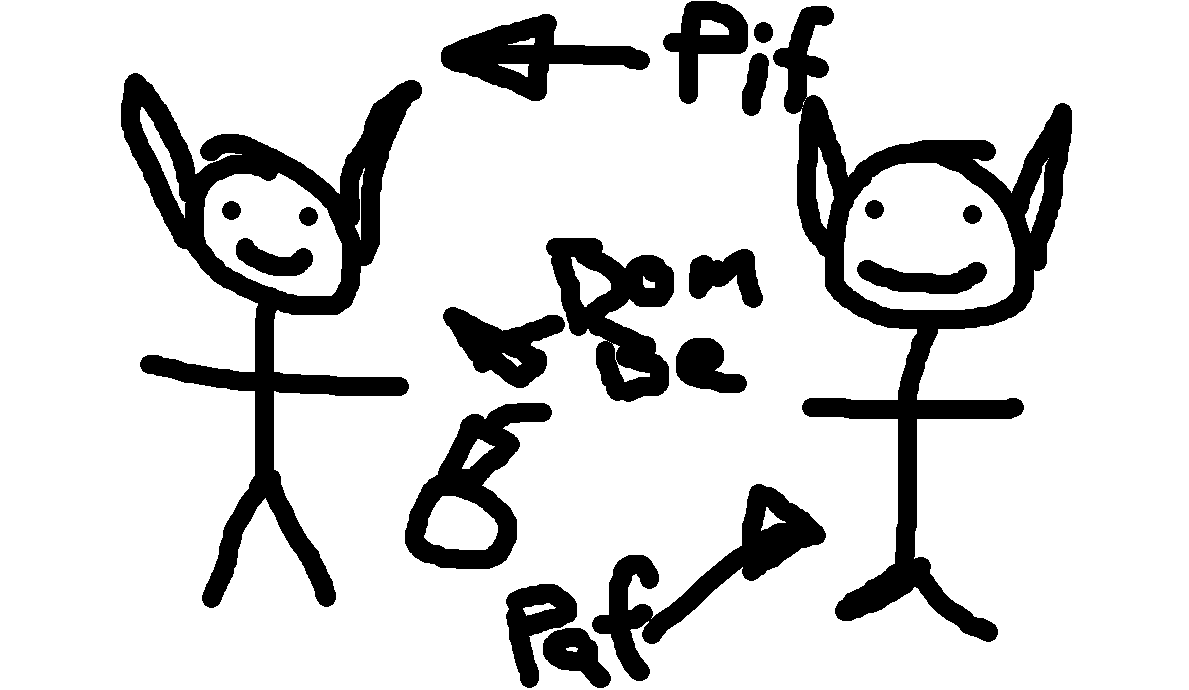
\includegraphics[width=0.9\textwidth]{PIFPAF.png}
\end{figure}
VI BRUG FOR SULFUR OG JERN TIL SPRINGE EVLER OP! DU BRING OS 5 JERN OG 5 SULFUR OG VI GIVE DIG SPECIEL PREMIE! DET VÆRE BOMBE I BREV! 
- PIF OG PAF!

\begin{center}
\fbox{
\begin{minipage}{0.9\linewidth}

\begin{center}
{\Large \textbf{KELLLWAN KIRKEN KALDER}}\\
\medskip
{\large \textit{Sydporten skal genopbygges}}
\end{center}

\par\medskip

Efter år med fejlslagne forsøg er arbejdet ved Sydporten nu begyndt under Kelllwan Kirkens ledelse. Men sten rejser sig ikke alene, og dæmonerne fra Letho venter ikke tålmodigt.

\par\medskip

Kirken søger derfor arbejdere, minefolk, eventyrere og ærlige borgere til indsamling af materialer til rigets forsvar.

\par\medskip

\begin{center}
\textbf{BETALING UDBETALES DIREKTE AF KELLLWAN KIRKEN}
\end{center}

\begin{center}
\Huge
10 Fjend for Jern\\
20 Fjend for Mitril
\end{center}

\par\medskip

Materialer afleveres ved Kelllwan Kirkens lejre nær Sydporten.

\par\medskip

Kun gennem handling sikres Kalish mod Lethos rædsler.


\end{minipage}
}
\end{center}
% ====== Handelskompagniets Kongetand-reklame ======
\begin{center}
\begin{tcolorbox}[
  enhanced,
  width=0.94\textwidth,
  colback=Goldenrod!7,
  colframe=Maroon!90!black,
  boxrule=1.6pt,
  borderline={0.6pt}{3pt}{Goldenrod!80!black},
  sharp corners,
  boxsep=2mm,
  left=6mm,
  right=6mm,
  top=5mm,
  bottom=5mm,
  overlay={
    % Dekorative hjørner
    \draw[Goldenrod!80!black,line width=1.3pt]
      ([xshift=2mm,yshift=-2mm]frame.north west)
      -- ++(14mm,0) -- ++(0,-7mm);

    \draw[Goldenrod!80!black,line width=1.3pt]
      ([xshift=-2mm,yshift=-2mm]frame.north east)
      -- ++(-14mm,0) -- ++(0,-7mm);

    \draw[Goldenrod!80!black,line width=1.3pt]
      ([xshift=2mm,yshift=2mm]frame.south west)
      -- ++(14mm,0) -- ++(0,7mm);

    \draw[Goldenrod!80!black,line width=1.3pt]
      ([xshift=-2mm,yshift=2mm]frame.south east)
      -- ++(-14mm,0) -- ++(0,7mm);

    % Lille segl øverst
    \node[
      circle,
      fill=Maroon!90!black,
      draw=Goldenrod,
      line width=1pt,
      minimum size=12mm,
      text=white,
      font=\sffamily\bfseries\scriptsize
    ] at ([yshift=-7mm]frame.north east) {HKG};
  }
]

% ----- Overskrift -----
\begin{center}
{\sffamily\bfseries\small\color{Maroon!90!black}
EN ENESTÅENDE MULIGHED FRA HANDELSKOMPAGNIET}

\vspace{0.25em}

{\sffamily\bfseries\fontsize{27}{29}\selectfont
\color{Maroon!90!black}
Bliv rig uden at arbejde!}

\vspace{0.3em}

{\color{Goldenrod!80!black}\rule{0.78\linewidth}{1.2pt}}
\end{center}

\vspace{0.5em}

Handelskompagniet giver dig en \textbf{eksklusiv mulighed} for at blive rig uden at løfte en finger!

\vspace{0.7em}

% ----- Hovedløftet -----
\begin{center}
\begin{tcolorbox}[
  width=0.82\linewidth,
  colback=Maroon!90!black,
  colframe=Goldenrod!80!black,
  boxrule=1.2pt,
  sharp corners,
  left=3mm,
  right=3mm,
  top=2.5mm,
  bottom=2.5mm
]
\centering
{\sffamily\bfseries\fontsize{21}{23}\selectfont\color{white}
Tjen op til \textbf{500 Fjend per dag}!}
\end{tcolorbox}
\end{center}

\vspace{0.3em}

Alt du skal gøre, er at samle \textbf{Kongetand}! Handelskompagniet opkøber i øjeblikket alle de kongetand, vi kan få fat i.

\vspace{0.5em}

Når du har bevist, at du kan samle 3 kongetand, får du \textbf{eksklusive rettigheder} til at oprette dit eget indsamlingskompagni!

\vspace{0.7em}

% ----- Trin-for-trin model -----
\begin{tcolorbox}[
  enhanced,
  colback=white,
  colframe=Goldenrod!70!black,
  boxrule=0.9pt,
  sharp corners,
  left=5mm,
  right=5mm,
  top=3mm,
  bottom=3mm,
  title={\sffamily\bfseries\large Sådan fungerer det:},
  coltitle=white,
  colbacktitle=Maroon!90!black,
  fonttitle=\sffamily\bfseries
]

\begingroup
\renewcommand{\labelitemi}{%
  \textcolor{Maroon!90!black}{\large\textbullet}%
}
\setlength{\itemsep}{0.45em}

\begin{itemize}
  \item Du samler 3 kongetander.
  \item Du finder 3 venner, der arbejder under dig.
  \item Hver af dem samler 3 kongetand til dig. Du har nu 9!
  \item Når de finder 3 venner hver, får du hele 36 kongetand!
\end{itemize}
\endgroup

\end{tcolorbox}

\vspace{0.7em}

% ----- Handelsrate -----
\begin{center}
{\sffamily\bfseries\small\color{Maroon!90!black}
HANDELSKOMPAGNIETS ATRAKTIVE HANDELSRATE}

\vspace{0.25em}

\fcolorbox{Maroon!90!black}{Goldenrod!18}{%
  \parbox{0.82\linewidth}{%
    \centering
    \vspace{0.35em}
    Med vores atraktive handelsrate tilbyder vi
    \textbf{\Large 5 HKG}\footnote{Handelskompagni Guld}
    per kongetand.
    \vspace{0.35em}
  }%
}
\end{center}

\vspace{0.7em}

Beviser du dit værd, bliver du udpeget til at være den officielle
\textit{"Viceformand for eksklusiv kongetandsdistribution og indsamling"}.\footnote{Bevis for denne titel koster 5000 HKG eller 50 Fjend.}

\vspace{0.8em}

% ----- Afsluttende opfordring -----
\begin{center}
\colorbox{Maroon!90!black}{%
  \parbox{0.88\linewidth}{%
    \centering
    \vspace{0.45em}
    {\sffamily\bfseries\large\color{white}
    Kontakt din lokale repræsentant for Handelskompagniet i dag!}
    \vspace{0.45em}
  }%
}
\end{center}

\vspace{0.35em}

\begin{center}
{\scriptsize\sffamily\itshape\color{black!65}
Handelskompagniet: Din indsats. Vores fremgang.}
\end{center}

\end{tcolorbox}
\end{center}


\separator



\begin{center}
\fbox{%
\begin{minipage}{0.9\linewidth}
\centering
\vspace{2em}
\resizebox{\linewidth}{!}{%
\begin{tikzpicture}
\path[
  decorate,
  decoration={
    text along path,
    text={|\Large\bfseries|KOM SPIS VED DEN TISSENDE NYMFE},
    text align=center
  }
]
(-6,0) arc[start angle=160, end angle=20, radius=6cm];

\useasboundingbox (-6,0) rectangle (6,1.4);
\end{tikzpicture}%
}

\vspace{-0.5em}

{\LARGE\bfseries KOM OVER TIL KROEN!}

\begin{itemize}
  \item ØL: 1 Fjend
  \item Mad: 2 Fjend
  \item Flaske: 10 Fjend
  \item God Stemning: 0 Fjend
\end{itemize}

\end{minipage}%
}
\end{center}


\begin{center}
\begin{tcolorbox}[
  enhanced,
  width=0.94\textwidth,
  colback=ForestGreen!4,
  colframe=black,
  boxrule=1.4pt,
  borderline={0.7pt}{3pt}{ForestGreen!70!black},
  sharp corners,
  boxsep=2mm,
  left=5mm,
  right=5mm,
  top=4mm,
  bottom=3mm,
  overlay={
    % Ornamenter i hjørnerne
    \draw[ForestGreen!70!black,line width=1.2pt]
      ([xshift=2mm,yshift=-2mm]frame.north west)
      -- ++(11mm,0) -- ++(0,-7mm);

    \draw[ForestGreen!70!black,line width=1.2pt]
      ([xshift=-2mm,yshift=-2mm]frame.north east)
      -- ++(-11mm,0) -- ++(0,-7mm);

    \draw[ForestGreen!70!black,line width=1.2pt]
      ([xshift=2mm,yshift=2mm]frame.south west)
      -- ++(11mm,0) -- ++(0,7mm);

    \draw[ForestGreen!70!black,line width=1.2pt]
      ([xshift=-2mm,yshift=2mm]frame.south east)
      -- ++(-11mm,0) -- ++(0,7mm);
  }
]

\begin{center}
{\sffamily\bfseries\small
TRÆT AF SVAGE GUDER OG TOMME LØFTER?}

\vspace{0.15em}

{\sffamily\bfseries\fontsize{28}{29}\selectfont
\textcolor{ForestGreen!55!black}{REJS DIG FOR ROHAR!}}

\vspace{0.1em}

{\sffamily\bfseries\large
KONGEN - DEN DER KOM TILBAGE}
\end{center}

\vspace{0.5em}

\noindent
\colorbox{black}{%
  \parbox{\dimexpr\linewidth-2\fboxsep\relax}{%
    \centering
    \color{white}
    \itshape\large
    ``Før var jeg træt og deprimeret, men så prøvede jeg
    at tilbede Rohar. Nu har jeg styrke, et formål og en
    gud, der råber gode råd gennem min økse!''
    
    \normalfont\small
    - Gruk Jernpande, tidligere Orlek Præst
  }%
}


\vspace{0.7em}

\begin{center}
\colorbox{ForestGreen!70!black}{%
  \parbox{0.88\linewidth}{%
    \centering
    \color{white}
    \sffamily\bfseries\large
    SPØRG EFTER ROHAR PRÆSTEN ELLER TEMPELKRIGEREN HVIS DU GERNE VIL VIDE MERE!

    \smallskip
    \normalsize
    Medbring jern, og alle dine fjend for at vise at du er værdig.
  }%
}
\end{center}

\vspace{0.4em}

\begin{center}
{\sffamily\bfseries
ROHAR DØDE. DET STOPPEDE HAM IKKE.\\
HVAD ER DIN UNDSKYLDNING?}
\end{center}


\end{tcolorbox}
\end{center}


\clearpage
\thispagestyle{newspaper}

\begin{center}
  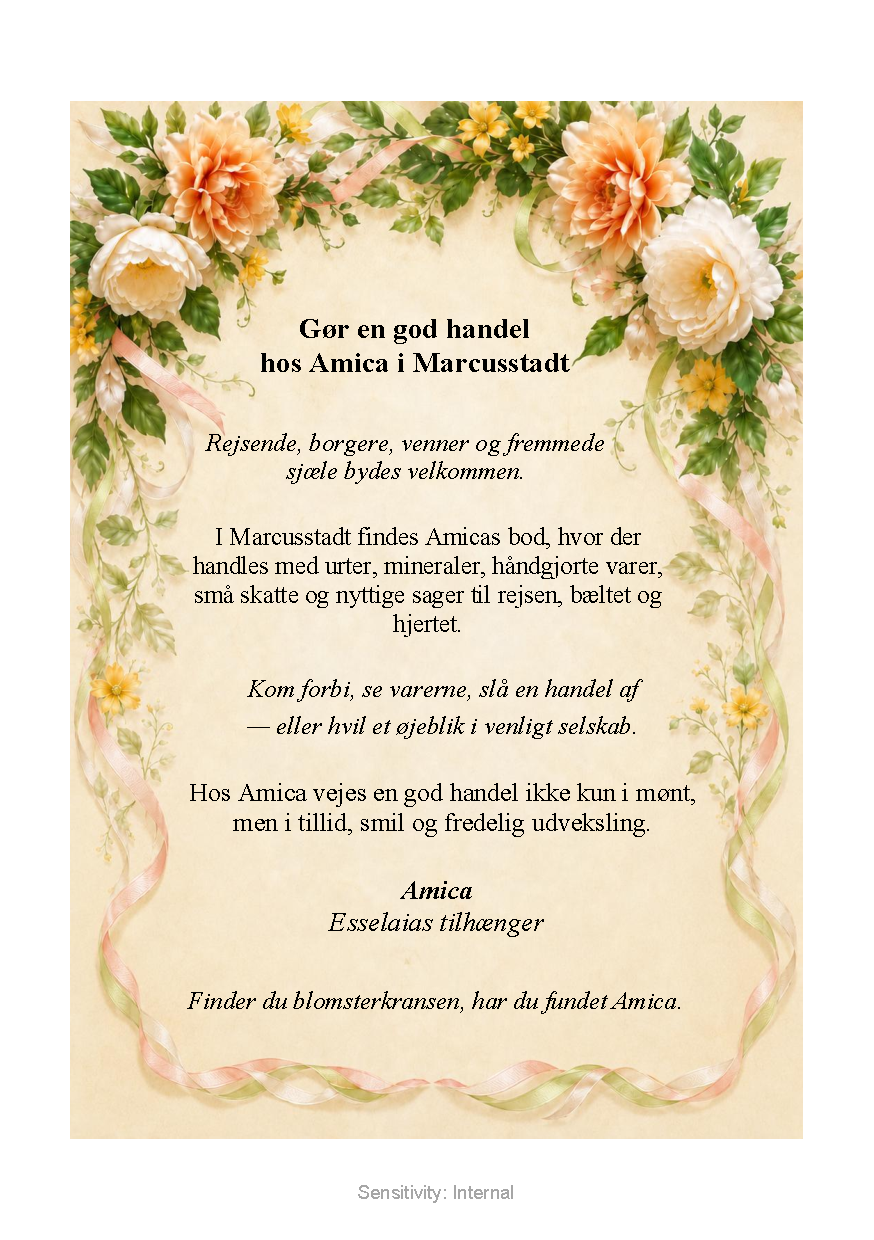
\includegraphics[
    width=\textwidth,
    height=0.96\textheight,
    keepaspectratio,
    trim={12mm 17mm 12mm 17mm},
    clip
  ]{artikel.pdf}
\end{center}

\end{document}